\newcommand{\institut}{Institut f\"ur Energie und  Automatisiertungstechnik}
\newcommand{\fachgebiet}{Elektronische Mess- und Diagnosetechnik}
\newcommand{\veranstaltung}{Praktikum Messdatenverarbeitung}
\newcommand{\pdfautor}{\"Ozg\"u Dogan (326 048), Timo Lausen (325 411), Boris Henckell (325 779)}
\newcommand{\autor}{\"Ozg\"u Dogan (326 048)\\ Timo Lausen (325 411)\\ Boris Henckell (325 779)}
\newcommand{\pdftitle}{Praktikum Messdatenverarbeitung  Termin 1}
\newcommand{\prototitle}{Praktikum Messdatenverarbeitung \\ Termin 1}
\newcommand{\aufgabe}{}

\newcommand{\gruppe}{Gruppe: G1 Fr 08-10}
\newcommand{\betreuer}{Betreuer: J\"urgen Funk}

\input{../../packages/tu_header_8}
%---------------------------------------------------------------------
%---------------------------------------------------------------------
%---------------------------------------------------------------------

\section{Vorbereitungsaufgaben}
\begin{quote}
	\subsection{Aufbau digitale Messkette}
    \begin{quote}
        Eine Digitale Messkette dient dem Zweck ein analoges Signal mit Hilfe eines Sensors zu erfassen und in ein
        Digitales Signal umzuwandeln.\\
        Konkret werden für die Messkette folgende Bauteile benötigt:
        \begin{itemize}
          \item Sensor
          \item Signalkonditionierung
          \item Anti-Aliasingfilter
          \item Abtast-Halte-Glied
          \item Analog-Digital-Umsetzer
        \end{itemize}
        Diese bearbeiten nacheinander das Eingangssignal.
        \begin{figure}[H]
			\centering
				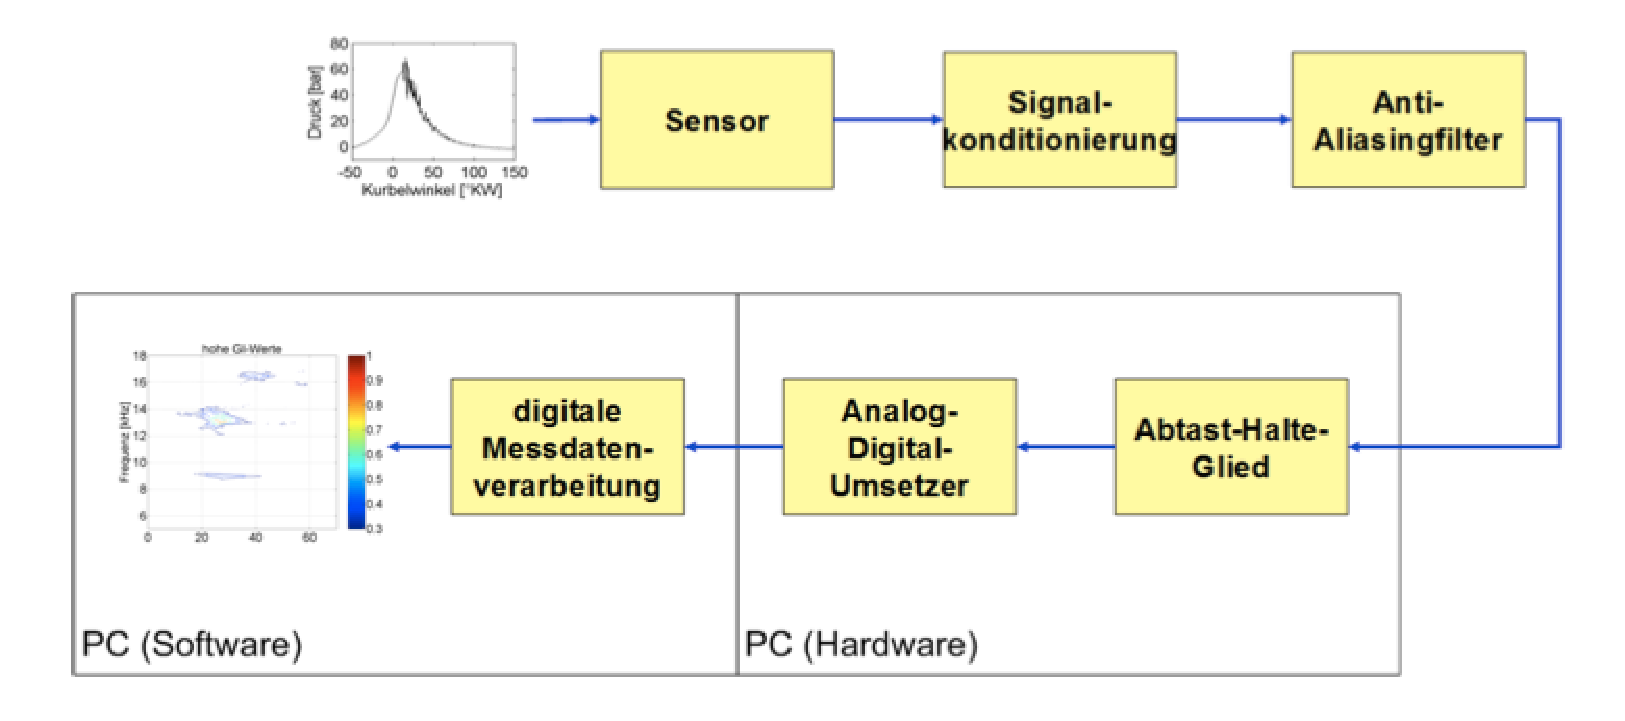
\includegraphics[scale=0.5]{DigitaleMesskette}
				   \caption{Digitale Messkette}
		\cite{DigitaleMesskette}
		\end{figure}
		\vspace{1em}
	 	
	 	Wir betrachten einige dieser Bauteile etwas genauer:
	 	\subsubsection{Signalkonditionierung}
		\begin{quote}
			Die Signalkontitioniertung hat das Ziel das Signal des Sensors an den Aussteuerbereich des Messystems anzupassen. Das
			kann bedeuten, dass das Signal verstärkt, gedämpft, gefiltert, linearisiert oder konvertiert werden muss. 
		\end{quote}
		\subsubsection{Anti-Aliasingfilter}
		\begin{quote}
		      Beim Abtasten eines Signals entsteht ein periodisches Spektum.Der Anti-Aliasingfilter hat die Aufgabe alle
		      Frequenzen die größer sind als die halbe Abtastfrequenz zu unterdrücken. Hierzu werden alle zu hohen Frequenzen von ihrer Amplitude auf einen Wert unterhalb des
              \"least significant bits\" gedämpft.
		      
		      \begin{equation*}
                	\begin{split}
                		\omega > \frac{\omega_0}{2} \hspace{2em} \text{mit} \hspace{2em} \omega_0 = \frac{2\pi}{T}
                	\end{split}
                \end{equation*}
		      
		      Würden diese Frequenzen nicht gefiltert werden würde es zu dem sogenannten Aliasing kommen bei dem höhere
		      Frequenzanteile fälschlicherweise als kleinere Frequenzen interpretiert werden. Als folge würde das
		      Originalsignal verfälscht weitergeleitet.\\
		      
		      Da ein abgetastetes Signal umso mehr dem Originalsignal ähnelt je höher die Abtastfrequenz ist, ist in diesem
		      Sinne eine möglichst hohe Abstastfrequenz erstrebenswert. Eine höhe Abstastfrequenz hat jedoch zur folge, dass
		      ein steilerer Anti-Aliasingfilter notwendig ist um das Aliasing zu verhindern. Außerdem ist die
		      Schaltungstechnische Umsetzung bald sehr herausfordernd.\\
		\end{quote}
		\subsection{Abtast-Halte-Glied}
        \begin{quote}
            Ein Abtast-Halte-Glied hat die Aufgabe einen Wert abzutasten und für die zeit zu halten die der ADU
            benötigt um aus dem Abgetasteten analogen Wert ein digitalen Wert zu konvertieren.
        \end{quote}
        \subsubsection{ADU}
		\begin{quote}
			Der Analog-Digital-Umsetzer ermittelt aus dem abgetasteten analogen Signal das dazupassende Digitale Signal.
		\end{quote}
    \end{quote}
\end{quote}

%--------------------------------------------------------------------
%--------------------------------------------------------------------

\section{Versuch}
\begin{quote}
	
\end{quote}

%--------------------------------------------------------------------
%--------------------------------------------------------------------

\section{Ergebnisse}
\begin{quote}
	
\end{quote}

%--------------------------------------------------------------------
%--------------------------------------------------------------------

\begin{thebibliography}{999}
\bibitem {DigitaleMesskette} Prof. Dr.-Ing. Gühmann, Clemens: MDVScript\_01, S.5

%Name, Vorname.; evtl. Name2, Vorname2.: Titel des Dokumentes
%oder Buches, Zeitschrift/Verlag/URL (Auflage, Erscheinungsort, -jahr), ggf. Seitenzahlen
%\bibitem [Wiki10] {DigitaleMesskette2} \url{www.wikipedia.org}, Zugriff 22.03.2010
\end{thebibliography}


\end{document}


